% !Mode:: "TeX:UTF-8"

\chapter{背景}[Background]

虽然目前很多公司都开发了自己的自动驾驶系统,但其使用的技术几乎都是基于计算机视觉,目标检测,目标识别等深度学习、机器学习技术。因此,针对自动驾驶系统的测试技术也是源于深度学习系统的测试技术。其中,在基于深度神经网络的自动驾驶系统中,其神经网络模型将被汽车的各种传感器(雷达、摄像头等)接收到的数据作为输入,经过神经元的运算处理后输出各种驾驶行为(方向盘拐角、刹车信号,速度控制信号等)。下图\ref{as_example}展示了一个机遇卷积神经网络的自动驾驶系统例子,这个系统由输入(摄像头拍摄的图像)、输出层(方向盘拐角)和中间的隐藏层组成。本章主要讲述传统的深度学习测试技术以及目前学术界比较推崇的自动测试技术。

\begin{figure}[h]
    \centering
    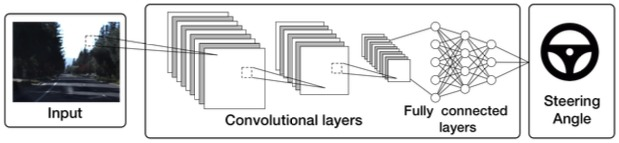
\includegraphics[width=0.8\textwidth]{as_example}
    \caption{基于卷积神经网络的自动驾驶系统\cite{DeepRoad}}
    \label{as_example}
\end{figure}

\section{传统的深度学习系统测试技术}[The traditional testing technology of DNN]

深度学习技术是一种通过研究同类大量数据的表征,对未知新数据的特征进行推测的一门技术。在其行使职能,即预测新数据特征前,必须要学习大量同类的数据,即模型训练。模型训练完成后为了提前检测模型的准确性,会在之前的训练数据集中保留一部分数据,作为训练结束后的模型的测试数据集,使其在未被学习过的测试数据集上进行预测,最后以测试数据集上的准确性作为训练好的模型的精准度。目前学术界公认理想的训练数据集与测试数据集占比分别为70\%和30\%。

% TODO 可扩展

数据集的具体数量跟模型处理的具体问题相关,一般来说,处理的问题越复杂,即数据的特征越多,需要的数据量也就越多,比如比较出名的ImageNet\cite{ImageNet}比赛,公开可用的数据集多达1500万张由人工标注的图片数据。深度学习技术对已有数据特征拟合的本质和其训练测试的过程导致其对数据量的严重依赖,传统的深度学习测试需要大量的人工收集、标注数据,着极度的增加了其中的人力成本。除此之外,传统的通过人工收集数据的方式有严重的缺点,即收集到的数据无法保证覆盖到了所有可能的极端场景,以自动驾驶测试数据集为例,人工收集的数据集一般是车载记录仪记录的道路驾驶视频图片,但一般大雨、大雪等极端天气场景数据很少也很难收集,这就给相应的极端场景自动驾驶系统测试带来了不确定性。

\section{DeepXplore、DeepTest和DeepRoad}[DeepXplore DeepTest and DeepRoad]

针对上诉问题,DeepXplore和DeepTest提出了深度学习系统测试用例自动生成系统来缓解深度学习系统对于数据量的依赖。

\subsection{DeepXplore}[DeepXplore]
DeepXplore首先指出了深度学习系统与传统的软件开发系统的不同:传统软件的开发人员直接指定软件系统的逻辑,然而深度学习则是从数据特征中“学习、推到”它们的运行规则,甚至对于深度学习系统的开发人员来说,他们都不一定清楚训练好的深度学习模型的确切运行逻辑。因此DeepXplore
不是直接寻找深度学习系统中的逻辑错误,而是通过自动产生、寻找一些能使多个同类深度学习系统做出不同行为判断的测试用例,然后并将这些找到的测试用例放回原训练数据集里重新训练模型,试图修正之前错误的行为

除了将使不同的DNN系统做出不同预测行为为目标外,DeepXplore也借鉴了传统软件测试技术中的代码覆盖率的概念,为了使得尽可能测试整个DNN系统,DeepXplore引入了神经元覆盖率的概念,即测试用例测试过程中,在整个深度学习系统中,被“激活”,即输出值超过了某个阀值,的神经元的个数占整个网络结构神经元总数的占比。与代码覆盖率类似,我们期望神经元覆盖率越高越好。

DeepXplore以神经元覆盖率和使得不同DNN系统输出不一致为目标,将在原始测试用例上的修改抽象成为一个优化算法,使用梯度上升算法,最后自动生成一些使得被测的DNN系统得到不同的预测值,且各个DNN系统的神经元覆盖率很高的测试用例,下图\ref{xplore-wf}是DeepXplore的工作原理图。

\begin{figure}[h]
    \centering
    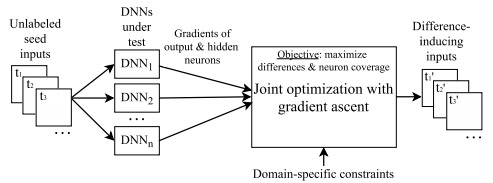
\includegraphics[width=0.8\textwidth]{xplore-wf}
    \caption{DeepXplore工作原理图\cite[图~5]{DeepXplore}}
    \label{xplore-wf}
\end{figure}

\subsection{DeepTest}[DeepTest]

DeepTest基于DeepXplore的工作,提出了一套专门针对自动驾驶系统,能够自动检测出错误行为的测试系统。发生在自动驾驶系统上的车祸大部分都是发生在一些罕见的路况场景下,而传统的自动驾驶检测测试技术几乎是完全依赖大量的罕见路况场景图片的人工收集与标注,这不仅包含了大量的人工成本,重要的是人工收集的数据无法保证能够覆盖度到了所有的极端场景数据。这些极端场景就好像是传统软件中的bug,但是这些bug一旦被检测到,就可能通过把这些导致错误的输入重新放入训练集,同时改变一下模型的结构和参数来修复。DeepTest正是通过以上的思路来设计的一套自动测试系统。

\begin{algorithm}[h]
    \small
    \SetAlgoLined
    \SetKwInOut{Input}{Input}
    \SetKwInOut{Output}{Output}
    \SetKwInOut{Variable}{Variable}

    \Input{变换Transformations T, 种子图像Seed Images I}
    \Output{合成的测试数据图像}
    \Variable{S: 存储新合成图像的栈; Tqueue: 存储变换的队列}

    push all seed imgs to Stack S; 所有种子图片入栈\;
    $genTests = \varnothing$\;
    \While{S is not empty}{
        img = S.pop()\;
        $Tqueue = \varnothing$\;
        numFailedTries = 0 \;
        \While{$numFailedTries \leq maxFailedTries$}{
            \eIf{$Tqueue\ is\ not\ empty$}{
                T1 = Tqueue.deque()
            }{
                Randomly pick transformations T1 from T
            }
            Randomly pick parameter P1 for T1\;
            Randomly pick transformation T2 from T\;
            Randomly pick parameter P2 from T2\;
            newImage = ApplyTransforms(image, T1, P1m T2, P2)\;
            \eIf{covInc(newiamge)}{
                Tqueue.enqueue(T1)
                Tqueue.enqueue(T2)
                UpdateCoverage()
                $genTests=genTests \cup newiamge S.push(newImaghe)$
            }{
                $numFailedTries=numFailed++$
            }
        }
    }
    return genTests
    \caption{混合变换优化算法\cite{DeepTest}}
    \label{alg1}
\end{algorithm}

具体的实现上,DeepTest依旧借用DeepXplore提出的神经元覆盖率的概念,使用位移、拉伸、仿射以及直接修改像素的透明度等基本的图形变换的手段来合成新的驾驶图像,文章里提到合成后的数据能使原DNN系统的神经元覆盖率提升100\%\cite{DeepTest},并以提升神经元覆盖率为目标,给出了一个优化算法\ref{alg1},以获得最佳的图像混合变换,最后DeepTest在利用这些合成的新数据重新训练自动驾驶模型来提高模型对于极端场景的鲁棒性。

\subsection{DeepRoad}[DeepRoad]

尽管DeepTest已经提出了一个较为完善的自动驾驶系统测试方案,以相对便宜和简洁的方法,利用大量的原始和合成出来的驾驶场景图片成功地检测出了许多自动驾驶系统前后不一致的驾驶行为,但它有一个很严重的缺陷:DeepTest用来合成图片的技术很难合成一些能够精确反映现实驾驶场景的图片,并且现实驾驶场景的图片也很难由一些基础的仿射、位移变换模拟合成出来,其用来模拟雨天、雾天的场景的技术仅仅是在原始图层上添加一层额外的图层,如下图\ref{deeptest_effect}所示,对于雾天,DeepTest仅仅是加了一层白色的图层,对于雨天,加了一层线条层。很明显这些合成图离现实中真实的驾驶场景有较大的差别。从另一个角度来说,即时用这些图检测出了自动驾驶系统错误的驾驶行为也很难有说服力,因为这些“出错”的场景在现实中根本不会出现。其实很多可能的真实的驾驶场景根本不能用一些简单的图像处理技术来模拟合成。

\begin{figure}[h]
    \centering
    \subfigure[DeepTest]{
        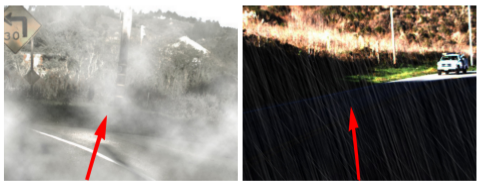
\includegraphics[width = 0.7\textwidth]{deeptest_effect}
    }
    \subfigure[DeepRoad]{
        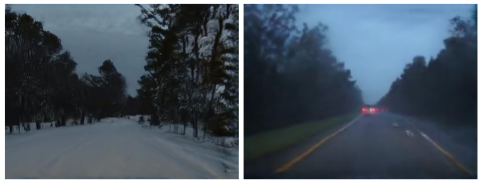
\includegraphics[width = 0.7\textwidth]{deeproad_effect}
    }
    \label{deeptest_effect}
    \caption{天气场景合成效果图比较}
\end{figure}

为了能够自动地合成大量真实的驾驶场景图片,DeepRoad提出了一个半监督合成的框架,抛弃了DeepTest用到的简单的图像处理技术来合成图像,采用深度学习对抗生成网络的技术来合成相对较真实的驾驶场景图片,上图\ref{deeptest_effect}为DeepTest合成图和DeepRoad使用对抗生成网络中UNIT\cite{UNIT}框架合成图的效果对比。可以清楚的看到使用UNIT技术合成的效果比较好的驾驶场景图已经与真实场景很接近了。下图\ref{deeproad_wf}展示了DeepRoad框架的整体流程。 

\begin{figure}[h]
    \centering
    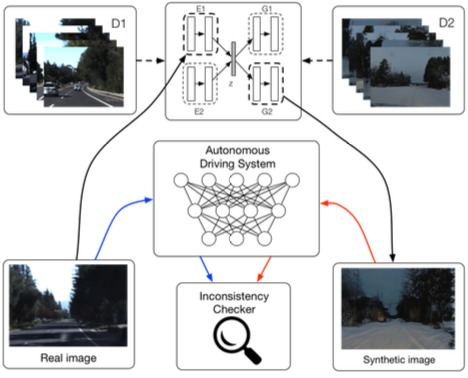
\includegraphics[width=0.75\textwidth]{deeproad_wf}
    \caption{DeepRoad框架流程图\cite{DeepRoad}}
    \label{deeproad_wf}
\end{figure}

DeepRoad将两种天气情况下的图片作为训练输入数据集,训练无监督对抗生成网络UNIT\cite{UNIT}框架,然后利用训练好的UNIT框架对未知新的输入数据进行转换合成,最后测试自动驾驶系统对使用UNIT进行转换后的图片做出的驾驶行为与未转换之前的原始图片的驾驶行为是否一致。

\section{其他的图像转换技术}[Other Image Transformation Technologies]

DeepRoad提出的将深度学习技术运用到自动驾驶系统测试用例合成,并设计的一套自动测试的框架在检测自动驾驶系统的稳定性和鲁棒性上,在其实验检测出了大量的现实自动驾驶系统有误的驾驶行为的结果\cite{DeepRoad}上看是有效的。其相对前人的工作DeepTest主要的改进是将测试用例的合成技术,即驾驶场景的图像转换技术,由原有的基本的图像变换换成了深度学习中的对抗生成网络技术。我们在利用UNIT合成驾驶场景图的实验过程中发现,虽然有效果比较好的合成图,但其占总的合成图的比例很小,1万张结果图中比较真实的图像大约有30多张,大部分的结果图如下,可以看到效果比较差,我们分析了效果比较差的原因主要是使用的训练数据集是由我们从Youtube上爬取的视频制作的数据图像,与UNIT官方使用的NVIDIA公司提供的闭源数据集相差比较大导致。

但其实目前学术界和工业界已经提出的能够进行不同天气场景图像转换的深度学习技术有很多,我们进行了调研,发现主要有两大类:对抗生成网络和图像风格转换(Neural Style Transfer)。我们对DeepRoad进行的实验也表明在得不到理想的训练数据集的情况下利用UNIT进行图像转换的实验结果是不理想的,那么可否将UNIT更换为其他的能够进行图像转换的深度学习技术?哪一种技术的实现效果是最好的?如何评价各种图像转换技术在合成驾驶场景图上的好坏?哪一种技术的训练成本和实现成本是最小的?针对以上问题,我们对现有的能够实现图像风格转换的深度学习技术展开实证研究,希望能够找到答案,最终可以为以后的自动驾驶系统测试人员在选择驾驶场景图片测试用例的合成技术框架上提供一些有帮助的建议。

% TODO UNIT图像

% word count ~ 3450

\chapter{实验}[Methodology]

% metrics -> intro of every gan and experiment, show results

为了尽可能地对所有能够实现图像风格变换的深度学习框架进行试验结果对比,我们首先调研了目前对图片合成图质量的量化评价指标,结合测试人员在实际测试过程中的各种成本以及实验细节,我们总结出了了3个指标: \textit{Fre ́chet Inception Distance(FID)}\cite{FID},模型训练时长以及自动驾驶系统对于前后合成图行为判断方向盘拐角差。

\section{评价指标}[Metrics]

对于图像驾驶场景合成图的质量好坏,最直观也是最直接的方式就是比较合成图的视觉效果,但这种人为的评判是主观且十分容易误判的。为了能够客观、量化的比较各个DNN框架合成的驾驶场景图的好坏,学术界提出了两个指标:\textit{Inception Score(IS)}\cite{IS}和\textit{Fre ́chet Inception Distance(FID)}\cite{FID}。

\textbf{Inception Score(IS).\cite{IS}}\quad IS评价合成图片质量是基于以下两点:(i) 包含有意义的物体图像的条件标记分布应该具有较低的熵(entropy)和(ii) 图像的多样性应该较高,进而边缘分布$\int_z p(y|x=G(z))dz$应该有较高的熵。
将以上两点汇总成一个评分,
\begin{center}
    $IS(G)=\exp{(E_{x\sim G}[d_{KL}(p(y|x), p(y)])}$
\end{center}
IS的作者用ImageNet\cite{ImageNet}的数据训练了一个分类器,最终实验结果反映IS的分数与人工标注评价正相关。

\textbf{Fre ́chet Inception Distance(FID).\cite{FID}}\quad FID提出了另一个评价方法,它首先将所有的合成图片放入一个特征空间,然后将该空间视为一个多元高斯分布,分别计算合成图和真实图的均值与方差,将两者高斯分布的Fre ́chet距离来量化真实图与合成图之间的距离,进而作为对合成图的评价:
\begin{center}
    $FID(x,g)=||\mu_x-\mu_g||_2^2+Tr(\sum_x + \sum_g - 2(\sum_x\sum_g)^{\frac{1}{2}})$
\end{center}
这里的$(\mu_x,\sum_x)$和$(\mu_g,\sum_g)$分别是数据分布和模型分布的均值和方差。FID的作者发现FID值与人类对合成图像的判断一直,并且较IS\cite{IS}鲁棒性更强。相对于IS,FID还能检测出不同类之间的区别,即如果每一种类别值产生合成一张图片,则很有可能获得比较高的IS分数,但对应的FID值却很低。基于以上几点,我们选用FID值而不选择IS值作为我们后面实验评价合成图片质量的评价指标之一。

\textbf{模型训练时长.}\quad 除了直接比较合成图片质量的好坏,在实际的自动驾驶系统测试过程中,我们还必须考虑到模型的训练时长。在选择理想的图片合成框架时,除了最终合成图片质量的好坏,我们还希望模型的训练时间成本尽可能的小,不同的模型根据不同的训练数据集大小,最终的训练时长也相差越大,比如本章后面会提到的UNIT\cite{UNIT}基于Udacity自动驾驶数据集\cite{udacity_dataset}和大约3000张驾驶场景图片,训练50万次时长大约一周左右。而对于一些图像风格转换(Neural Style Transfer)模型来说,训练时长却只要几个小时,虽然最后合成图的质量不如UNIT,但我们希望把这些数据都统计出来,具体的取舍留给实际最终的测试人员自己选择。 

\textbf{方向盘拐角差.}\quad 有了合成图质量的量化指标,模型的训练时间成本比较,最后我们还希望直观地看到合成图相比原始图对于自动驾驶系统行为判断(方向盘拐角信号)的影响。理想情况下,只变换驾驶场景图片的风格,比如晴天的路况转换为夜晚、雨天或者阴天的路况,自动驾驶系统对于大部分的转换后的图像的行为判断,即输出的方向盘拐角信号,与原始的驾驶路况图片做出的行为判断应该几乎一致,或者差别不大。实验中我们对两者的信号,即拐角差设置了一个阈值$\alpha=5^{\circ}$,我们希望小于阈值的图片占比越小越小,最后我们以两者之间拐角差的方差作为该指标的量化数据。

综上述,在后面的实验中,我们将统计所有实验模型的\textbf{FID值}、\textbf{模型训练时长}和\textbf{方向盘拐角差}3个指标。

% wc ~ 1400

\section{模型的筛选与实验}[Model Filting and Experiments]

基于DeepRoad的工作,我们首先选择实验的DNN模型大类是对抗生成网络\cite{GAN},因为其生成仿照数据的功能契合我们对于合成驾驶场景图片的需求,下面简单的介绍一下对抗生成网络的背景以及选择的对应模型。

\subsection{对抗生成网络大类}[Generative Adversarial Network Class]

对抗生成网络\cite{GAN}首先由Ian J. Goodfellow等人提出,它的本质是模拟真实数据源的概率分布。其基本框架有两个神经网络组成:生成模型网络和判别模型网络,其中判别模型负责学习区分数据是否来自真实数据分布,而生成模型可以想象成一个制造伪币的团伙,试图产生能够通过货币监测的钞票,判别模型正是这个对抗游戏中的警察,试图甄别出货币中的假钞。整个对抗生成网络模型的训练过程就是对抗模型和生成模型的训练竞赛,整个训练过程直到判别模型再也区分不出数据是来自真实数据分布还是生成模型伪造的数据为止。

训练过程中,对抗模型一般使用向后传播算法,而判别模型一般使用向前传播算法。其中判别模型为了通过数据$x$学习生成器的数据分布$p_g$,可以基于输入的噪声数据定义一个先验概率$p_z(z)$,然后将整个数据空间表示为$G(Z;\theta_g)$,这里的$G$是一个参数为$\theta$的多层神经网络可微函数。再定义一个输出为一个单向量的多层神经元网络$D(x;\theta_d)$,其中$D(x)$表示数据$x$来自真实数据而非$p_g$的概率。我们训练$D$直到我们对所有数据正确标记其是否来自判别器的概率最大为止。同时也训练$G$来最小化$\log(1-D(G(z)))$。上述可总结成下面的公式:
\begin{equation}
    \label{eq:gan}
    \min_G\max_DV(D,G)=\xi_{x\sim p_{data}(x)}[\log D(x)]+\xi_{z\sim p_z(z)}[\log(1-D(z))]
\end{equation}
实际训练过程中,等式\eqref{eq:gan}中的生成器$G$可能会出现梯度消失的问题,但由于本文章不是对对抗生成网络算法的研究,所以就不在此展开了。

为了对目前所有的对抗生成网络技术能有一个综合的认识,我们主要参考了文献\cite{gan-survey},跟据文献中的分类,依次对每种类型中比较典型的框架进行了实验与数据总结统计。实验过程中为了保持尽量跟框架作者实现的效果性能一致,我们只选取了提供了源代码的框架进行了实验。

% TODO: confirm this
\textbf{统一说明},本文后续所有的实验均是在64位Ubuntu 16.04.6 LTS操作系统,8核GTX 1080ti-GPU硬件环境下进行的。

\subsubsection{DCGAN}[DCGAN]

\textbf{DCGAN.}\cite{dcgan}\quad 是一个深度卷积对抗生成网络,其生成器和判别器使用的是限制卷积网络,主要的架构特点有:(1)用多步卷积和分布卷积层代替了所有的池化层(pooling layer);(2)使用了批量统一化层(batch normalization layer);(3)去掉了所有的全连接层;(4)在生成器中,使用$\tan{h}$作为输出层的激活函数,ReLU函数作为其它层的激活函数;(5)判别器中,所有层的激活函数都使用LeakyReLU函数。

虽然DCGAN的作者将其运用在人脸合成与转换上相当成功,但我们后来将其训练集换成了Udacity的自动驾驶路况数据集以及youtube上爬取的数据,实验结果样本图如下图\ref{dcgan_example}所示,效果却不理想。

\begin{figure}[t]
    \centering
    \subfigure[DCGAN在人脸图像合成的效果样例图]{
        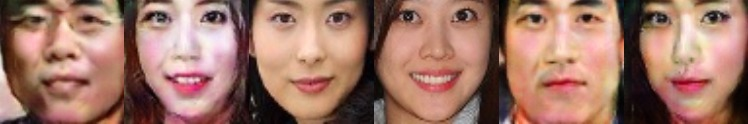
\includegraphics[width=0.75\textwidth]{dcgan_example}
    }
    \subfigure[DCGAN在自动驾驶数据集上的效果样例图]{
        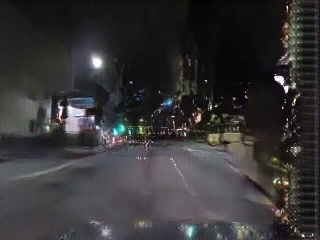
\includegraphics[width=0.4\textwidth]{results/dcgan_night}
        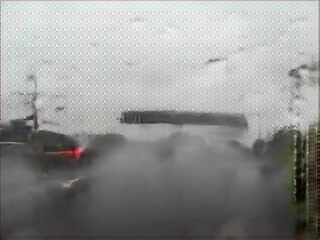
\includegraphics[width=0.4\textwidth]{results/dcgan_rain}
    }
    \caption{}
    \label{dcgan_example}
\end{figure}

实验代码使用的是\cite{dcgan}论文中给出的代码,其中主要参数配置如下

\begin{lstlisting}[basicstyle=\small]
    --bathSize     200          // 批量实验数据大小
    --imageSize    180, 320     // 设置图像尺寸大小
    --nz           20           // z向量
    --niter        10000        // 训练的次数
    --lr           0.0002       // Learning rate
    --cuda                      // 在cuda库上训练
\end{lstlisting}

由于DCGAN在驾驶路况图片上的合成效果很差,于是我们放弃了对该框架进一步的实验结果数据统计与总结。

% wc ~ 1200

\subsubsection{CycleGAN}[CycleGAN]

\textbf{CycleGAN.}\cite{CycleGAN}\quad 该模型的本质是学习不同图片类(比如晴天和雨天)的数据分布映射函数。给定两个不同类的数据集$X$和$Y$以及训练样本集$\{x_i\}_{x=1}^N, \{y_j\}_{j=1}^M$,其中$x_i\in X, y_j\in Y$。将数据分布记为$x\sim p_{data}(x), y\sim p_{data}(y)$。如图\ref{cyclegan_1}所示,CycleGAN包含两个映射函数$G: X\to Y$和$F: Y\to X$,其次,CycleGAN还引进了两个判别器$D_X$和$D_Y$,其中$D_X$的目标是区分图像集$\{x\}$和转换的图像集$\{F(y)\}$,同样的,$D_Y$的目标是区分图像集$\{y\}$和$\{G(x)\}$。最终模型的训练目标是得到两个损失函数:(i)对抗损失函数,可以将合成的图像数据分布匹配对应到目标类的数据分布上;(ii)循环一致损失函数,阻止之前学习到的两个映射函数$G$和$F$彼此相矛盾。

\begin{figure}[h]
    \centering
    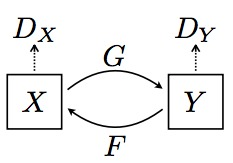
\includegraphics[width=.35\textwidth]{cyclegan_1}
    \label{cyclegan_1}
    \caption{}
\end{figure}

CycleGAN将对抗损失应用到了两个映射函数上,对于映射函数$G:X\to Y$和他的判别器$D_Y$,可以将其目标函数表示为
\begin{align*}
    \label{eq:2}
    \centering
    L_{GAN}(G,D_Y,X,Y)= & \xi_{y\sim p_{data}(y)}[\log D_Y(y)] + \\
    & \xi_{x\sim p_{data}(x)}[\log (1-D_Y(G(x)))]
\end{align*}

这里的$G$试图产生类似于类$Y$的图像集$G(x)$,然而$D_Y$的目标是区分转换的图像$G(x)$和真实的图像数据$y$。$G$旨在与对抗器$D$竞争最小化该目标函数。

对抗器理论上可以训练出可以输出和目标类$Y$与$X$分布完全相同的数据的映射函数$G$和$F$,但是如果网络的体积足够大,可以将相同的输入图片集映射到目标图片类的任意图像子集里。因此,单靠对抗损失函数无法保证学习到了映射函数能将单张输入图片$x_i$映射到理想的输出$y_i$。为了进一步减小可能的映射函数空间,CycleGAN提出循环一致映射函数,即对于来自类$X$的每张图像,对应的图像转换循环应该能够将$x$转换成原始图片,即\textit{向前循环一致}。上述的循环一致损失函数可以表示为:
\begin{align*}
    \label{eq:3}
    \centering
    L_{cyc}(G,F)= & \xi_{x\sim p_{data}(x)}[||F(G(x))-x||_1] + \\
    & \xi_{y\sim p_{data}(y)}[||G(F(y))-y||_1]
\end{align*}

综合等式\ref{eq:2}和等式\ref{eq:3}我们可以得到总的目标函数:
\begin{align*}
    \centering
    L(G, F, D_X, D_Y) = & L_{GAN}(G,D_Y, X, Y) \\
    & + L_{GAN}(F,D_X, Y, X) \\
    & + \lambda L_{cyc}(G, F)
\end{align*}
这里的$\lambda$控制着两个目标的相对重要性。下图是我们将CycleGAN运用在我们的数据集上,进行了晚上到白天以及黑天场景转换的实验结果样本图。

\begin{figure}[h]
    \centering
    \subfigure[原始图片]{
        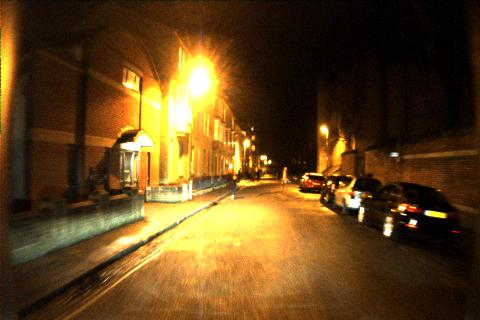
\includegraphics[width=0.3\textwidth]{results/cyclegan-input}
    }
    \subfigure[白天场景]{
        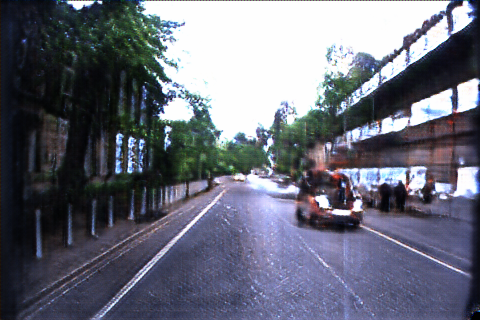
\includegraphics[width=0.3\textwidth]{results/cyclegan-sun}
    }
    \subfigure[黑天场景]{
        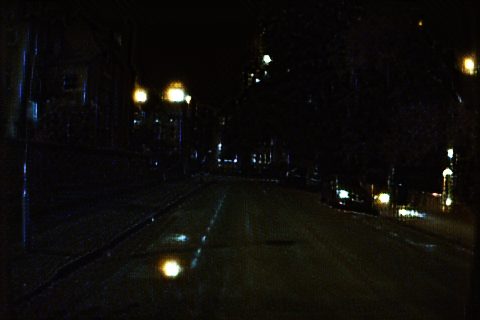
\includegraphics[width=0.3\textwidth]{results/cyclegan-night}
    }
    \caption{CycleGAN实验样例图}
\end{figure}

% wc ~ 800

\subsubsection{MUNIT}[MUNIT]

\textbf{MUNIT.}\cite{MUNIT}\quad MUNIT是基于UNIT\cite{UNIT}工作的进一步优化。它提出了一个可以解决多模型图片到图片转换问题的框架。它对于图像转换问题提出了几个假设:图片的潜在空间(latent space)可以被分解成内容空间和样式空间。基于上一个假设又提出了不同域类的图片共享一个类似的内容空间,但样式空间不一致。为了将一张图片转换成目标域类,MUNIT提出可以将图片的内容码与目标域类样式码空间的一个随机样式码重组。这里的内容码代表了在图片转换过程中应该被保留的信息元,而状态码则代表了不包含在输入图片中还剩下的变量元。通过采样不同的状态码,MUNIT模型能够产生多样,多模型的输出。以上严格的数学定义如下:

假定$x_1\in \chi_1$和$x_2\in \chi_2$是来自两个图片域类的图片集,给定来自两个不同边缘分布$p(x_1)$和$p(x_2)$的样本图片集,但不知道联合分布$p(x_1, x_2)$。MUNIT的目的是利用学习到的图片到图片转换模型$p(x_{1\to 2}|x_1)$和$p(x_{2\to 1}|x_2)$来预测两个边缘分布$p(x_1|x_2)$和$p(x_2|x_1)$,这里的$x_{1\to 2}$是由将$x_1$转换成$x_2$产生的一个样本输出。一般来说,$p(x_1|x_2)$和$p(x_2|x_1)$通常是十分复杂且多模型分布,为了简化这两个边缘分布,MUNIT提出了\textit{部分共享潜在空间假设}。即假设每张图片$x_i\in \chi_i$都是由两种码,内容码和样式码,组成,其中内容码$c\in C$由两个类域共享,而样式码$s_i\in S_i$则是每个域类图片所特有的。换句话说,一组来自联合分布的对应的图片$(x_1, x_2)$是由$x_!=G_1^*(c,s_1)$和$x_2=G_2^*(c, s_2)$生成的,这里的$c,s_1,s_2$都是来自鲜艳分布,$G_1^*,G_2^*$是实际的生成器。进一步假设$G_1^*$和$G_2^*$是确定性函数,且有反解码器$E_1^*=(G_1^*)^{-1}$和$E_2^*=(G_2^*)^{-1}$。MUNIT的目的是利用神经网络学习实际的生成器以及编码函数。它使用了两个重建的目标函数:给定来自数据分布的图像样本,在编码和解码后我们能够重建它:
$$L_{recon}^{x_1}=E_{x_1\sim o(x_1)}[||G_1(E_1^c(x_1), E_1^s(x_1))-x_1||_1] $$

给定在转换时的样式和内容码,我们也应该能够在解码和编码后重建图像:
\begin{align*}
    L_{recon}^{c_1}= & E_{c_1\sim p(c_1), s_2\sim q(s_2)}[||E_2^c(G_2(c_1,s_2))-c_1||_1] \\
    L_{recon}^{s_2}= & E_{c_1\sim p(c_1), s_2\sim q(s_2)}[||E_2^s(G_2(c_1, s_2))-s_2||_1]
\end{align*}

结合以上公式,MUNIT的总的损失函数可以由下面的公式表示:
\begin{gather*}
\min_{E_1,E_2,G_1,G_2}\max_{D_1,D_2}L(E_1,E_2,G_1,G_2,D_1,D_2)=L_{GAN}^{x_1}_L_{GAN}^{x_2}+\\
\lambda_x(L_{recon}^{x_1}+L_{recon}^{x_2})+\lambda_c(L_{recon}^{c_1}+L_{recon}^{c_2})+\lambda_s(L_{recon}^{s_1}+L_{recon}^{s_2})
\end{gather*}

最后我们使用了MUNIT提供的代码,进行了晴天路况图和雪天场景的转换,主要的优化配置参数如下和最终的实验结果样例图如下:

\begin{lstlisting}[basicstyle=\small, caption={MUNIT主要优化参数配置}, captionpos=b]
    max_iter: 1000000             # maximum number of training iterations
    batch_size: 1                 # batch size
    weight_decay: 0.0001          # weight decay
    beta1: 0.5                    # Adam parameter
    beta2: 0.999                  # Adam parameter
    init: kaiming                 # initialization [gaussian/kaiming/xavier/orthogonal]
    lr: 0.0001                    # initial learning rate
    lr_policy: step               # learning rate scheduler
    step_size: 100000             # how often to decay learning rate
    gamma: 0.5                    # how much to decay learning rate
    gan_w: 1                      # weight of adversarial loss
    recon_x_w: 10                 # weight of image reconstruction loss
    recon_s_w: 1                  # weight of style reconstruction loss
    recon_c_w: 1                  # weight of content reconstruction loss
    recon_x_cyc_w: 10             # weight of explicit style augmented cycle consistency loss
    vgg_w: 0                      # weight of domain-invariant perceptual loss
\end{lstlisting}

\begin{figure}[h]
    \subfigure[原始图片]{
        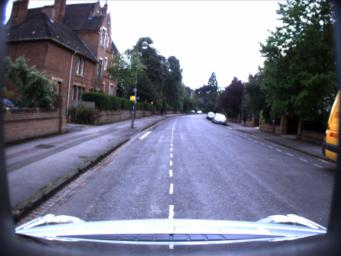
\includegraphics[width=.3\textwidth]{results/munit}
    }
    \subfigure[雪天场景1]{
        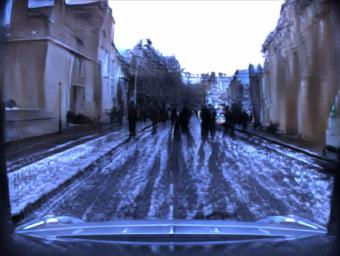
\includegraphics[width=.3\textwidth]{results/munit_winter}
    }
    \subfigure[雪天场景2]{
        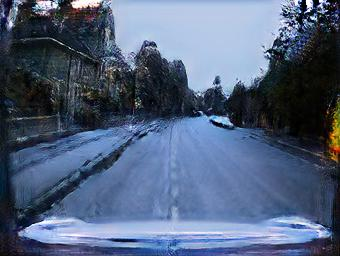
\includegraphics[width=.3\textwidth]{results/munit_winter2}
    }
    \caption{MUNIT实验样例图}
\end{figure}

\subsubsection[EBGAN]{EBGAN}

\textbf{EBGAN.}\cite{ebgan}\quad 的核心思想是讲判别器视为一个能量函数而不是通常的概率函数。它提出了对抗生成模型训练的一个基于能量表达的公式。由判别器计算出来的能量函数可以被视作生成器的可训练代价函数。虽然可以将能量函数通过Gibbs分布转换成概率函数,但是基于它提出的基于能量形式的对抗生成网络由于缺少归一化,从而使我们在判别器的架构和训练过程中有了更多的选择,下面简单阐述一下EBGAN的基本原理。

将$p_{data}$视作产生真实数据集分布的概率密度函数,生成器$G$训练生成赝本数据$G(z)$。为了定义能量函数,判别器的输出通过一个目标泛函算子进行转换,将低能量视为真实样本数据,而高能量则为合成的伪数据。跟一般的对抗生成网络一样,EBGAN也使用了两个不同的损失函数来分别训练生成器和判别器。

给定一个正边缘分布函数$m$,一个数据样本$x$和一个生成样本$G(z)$,判别器损失函数$L_D$和生成器损失函数$L_G$可以定义为以下:
\begin{align*}
    L_D(x, z) = & D(x) + [m - D(G(z))] \\
    L_G(z) = & D(G(z))
\end{align*}

给定一个生成器$G$,$p_G$为$G(z)$的密度分布,这里$z\sim p_z$。换句话说,$p_G$是由$G$产生的样本的概率密度函数。定义$V(G,D)=\int_{x,z}L_D(x,z)p_{data}(x)p_z(z)dxdz$和$U(G,D)=\int_zL_G(z)p_z(z)dz$,训练中判别器来最小化$V$值,生成器最小化$U$值。该系统的纳什均衡是一组满足一下条件的一对$(G^*,D^*)$:
\begin{align*}
    V(G^*,D^*) \leq V(G^*,D) \quad\quad \forall D \\
    U(G^*,D^*) \leq U(G,D^*) \quad\quad \forall G
\end{align*}

我们在已有的数据集上使用了tensorflow实现的EBGAN代码\cite{ebgan-github},实现了晴天路况到雨天场景的转换,以下是实验结果样例图

\begin{figure}[h]
    \centering
    \subfigure[原始图片]{
        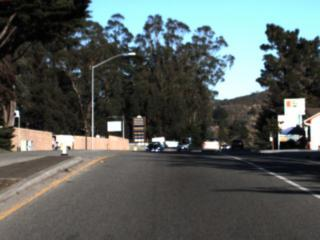
\includegraphics[width=.45\textwidth]{results/ebgan-input}
    }
    \subfigure[雨天场景]{
        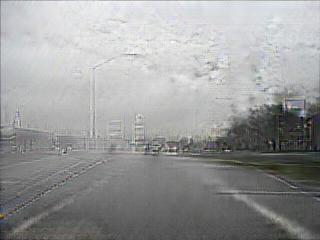
\includegraphics[width=.45\textwidth]{results/ebgan-rain}
    }
    \caption{}
\end{figure}

% wc ~ 1700

\subsection{图像风格转换大类}[Neural Style Transfer Class]

图像风格转换技术是受启发于近20年来卷及网络神经的发展,Gatys等人\cite{nst}提出利用卷积神经网络来复现一些著名的绘画风格。为了获得输入图片的风格表征形式,他们使用了一个原本用来获取图层信息的特征空间。该特征空间构建于神经网络的每一层过滤网之上。它由特征图谱各个部分的过滤网之间的协方差组成。通过引进多层网络之间的特征协方差,可以得到一个输入图片的一个静止、多尺度的能够包含图层信息的表征形式。再者,还可以通过构建一张匹配给定的输入图片的样式表达的图片来将建立在网络中不同层的样式特征空间信息可视化。为了合成拥有输入图片样式的图片,一般的图像风格转换技术会最小化来自一层网络的内容表征的白噪声图片与卷积网络层中输入图片的样式表征之间的距离。让$\overrightarrow{p}$表示合成照片,$\overrightarrow{a}$表示输入图片,则损失函数可以表示为:
$$
\centering
L_{total}(\overrightarrow{p},\overrightarrow{a}, \overrightarrow{x})=
\alpha L_{content}(\overrightarrow{p}, \overrightarrow{x}) +
\beta L_{style}(\overrightarrow{a}, \overrightarrow{x})
$$

这里的$\alpha$和$\beta$分别表示内容和样式在重建过程中的权重。下面我们参考了文献\cite{nst-survey},根据里面给出的分类抽取了具有代表性的几个模型进行了实验,实验平台跟之前的实验一致。

\subsubsection[AdaIN-style]{AdaIN-style}

\textbf{AdaIN-style.}\cite{adain}\quad 文献\cite{ioffe}提出批量正则化层极大的简化了向前传播网络的训练,AdaIN-style的模型结构也使用了批量正则化层,并且在次基础上通过将该层的激活函数改为单例正则,训练性能得到的巨大提升:
$$ IN(x)=\gamma(\frac{x-\mu(x)}{\tau(x)})+\beta$$
与之前的批量正则层不同的是单例层在测试阶段不变,然而批量正则层通常会用总体统计数据替换掉批量神经元的均值。

除了学习仿射参数$\gamma$和$\beta$,另一个改进方式是为每一个样式$s$学习不同的参数$\gamma^*$和$\beta^*$:
$$CIN(x;s)=\gamma^*(\frac{x-\mu(x)}{\tau(x)})+\beta^*$$
训练过程中,样例图片和它的指数$s$被随机从一个固定的样例集合$s\in {1,2,\dots,S}(S=32)$选取。内容图片会被样式转换网络进行转换,该网络中对应的$\gamma^*$和$\beta^*$被用在条件单例正则层里。

总体来说,AdaIN通过转换特征统计量,特别是像素均值和方差,来实现特征空间的样式转换。
AdaIN在已有的数据集上晴天转雪天、晚上的实验结果样例图如下:
\begin{figure}[h]
    \centering
    \subfigure[]{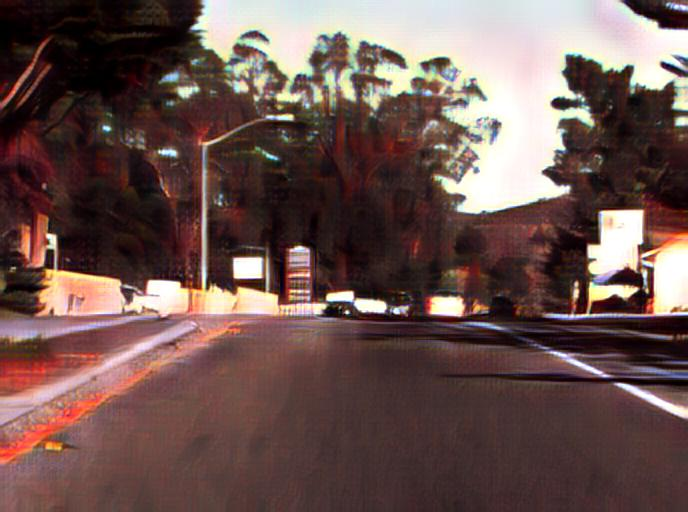
\includegraphics[width=.23\textwidth]{adin/adin1}}
    \subfigure[]{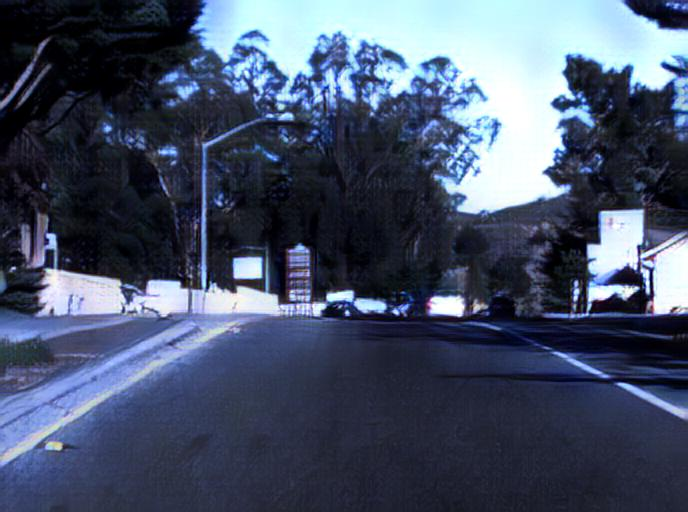
\includegraphics[width=.23\textwidth]{adin/adin2}}
    \subfigure[]{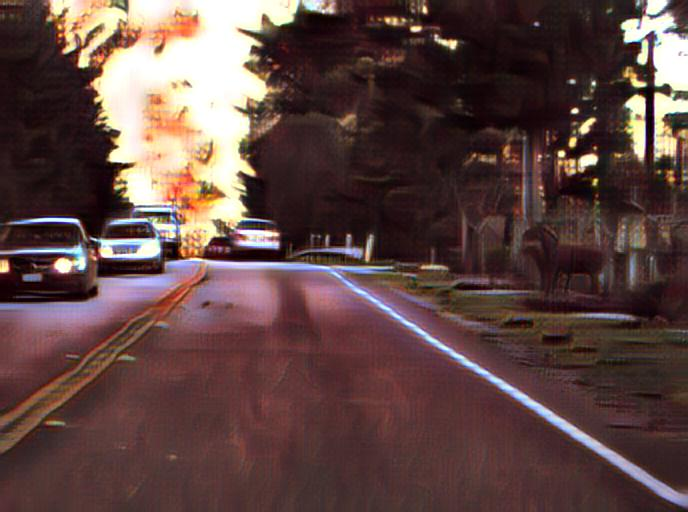
\includegraphics[width=.23\textwidth]{adin/adin3}}
    \subfigure[]{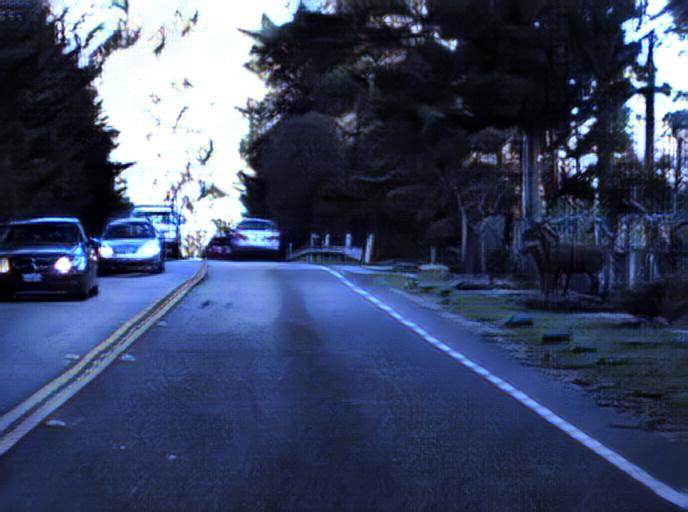
\includegraphics[width=.23\textwidth]{adin/adin4}}
    \caption{AdaIN实验结果样例图}
\end{figure}

% wc ~ 800

\subsubsection{Deep Photo Style Transfer}[Deep Photo Style Transfer]

\textbf{Deep Photo Style Transfer.}\cite{dpst}\quad  

\subsubsection{Fast Photo Style}[Fast Photo Style]

\textbf{Fast Photo Style.}\cite{fps}\quad  

\chapter{发现}[Findings]

\chapter{相关研究}[Related Work]

\chapter{总结}[Conclusions]